\begin{figure*}[t]
  \centering
  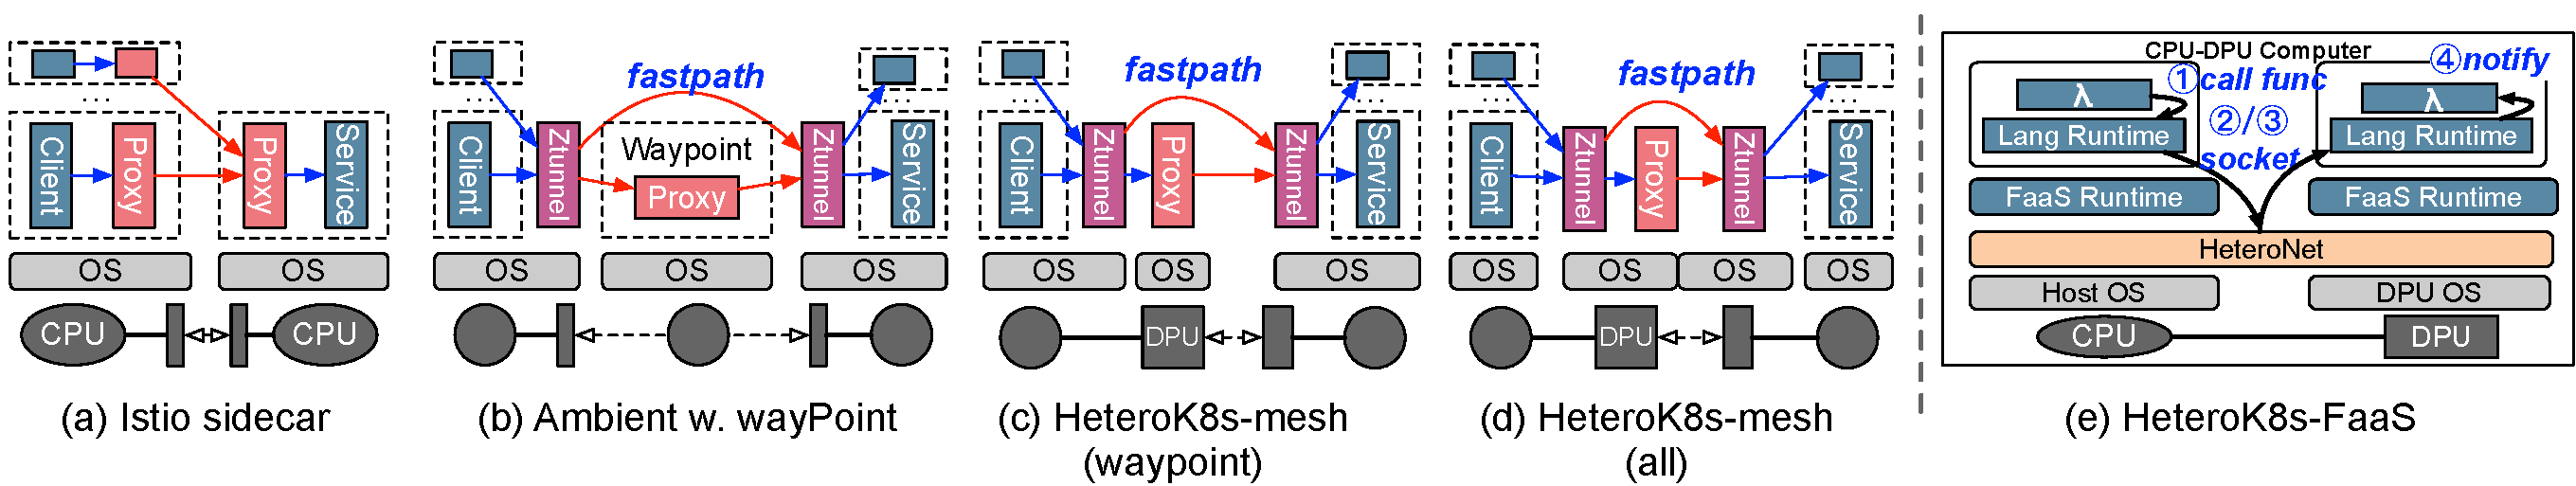
\includegraphics[width=0.96\textwidth]{figs/intro-wingman-compare-eps-converted-to.pdf}
  \caption{采用不同体系结构的服务网格（a/b）、\mesh（c/d）和 \faas（e）。}
  \label{fig:intro-wingman}
\end{figure*}

\begin{figure*}[t]
  \centering
  \begin{minipage}[t]{0.48\linewidth}
    \centering
    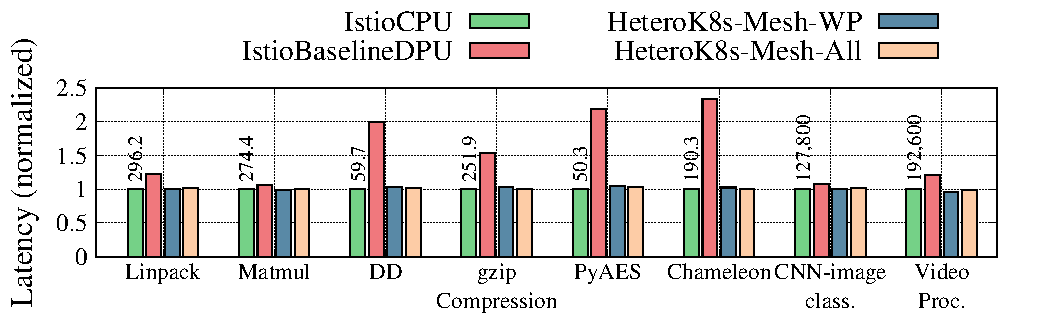
\includegraphics[width=0.98\linewidth]{figs-eval/eval-mesh-e2e-funcbench-eps-converted-to.pdf}\\[-0.4ex]
    \footnotesize\textbf{（a）FuncBench。}
  \end{minipage}
  \begin{minipage}[t]{0.48\linewidth}
    \centering
    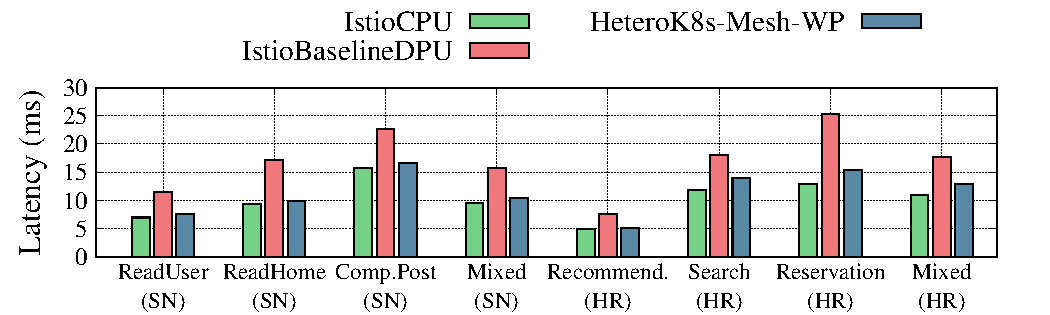
\includegraphics[width=0.98\linewidth]{figs-eval/eval-mesh-e2e-deathstar-eps-converted-to.pdf}\\[-0.4ex]
    \footnotesize\textbf{（b）DeathStarBench。}
  \end{minipage}

  \begin{minipage}[t]{0.235\linewidth}
    \centering
    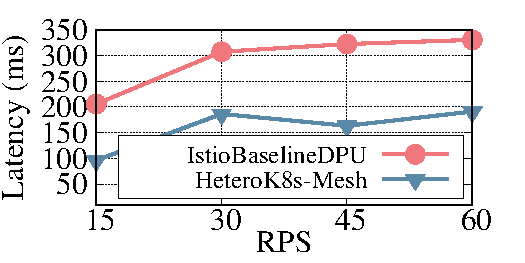
\includegraphics[width=0.98\linewidth]{figs-eval/eval-mesh-scale-avg-eps-converted-to.pdf}\\[-0.4ex]
    \footnotesize\textbf{（c）平均延迟。}
  \end{minipage}
  \begin{minipage}[t]{0.235\linewidth}
    \centering
    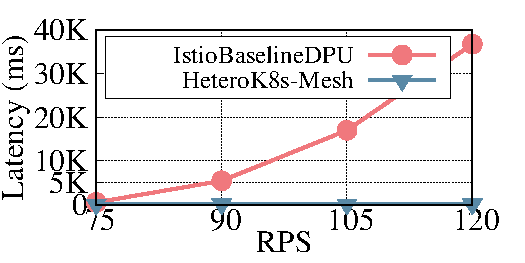
\includegraphics[width=0.98\linewidth]{figs-eval/eval-mesh-scale-avg-large-eps-converted-to.pdf}\\[-0.4ex]
    \footnotesize\textbf{（d）平均延迟（高 RPS）。}
  \end{minipage}
  \begin{minipage}[t]{0.235\linewidth}
    \centering
    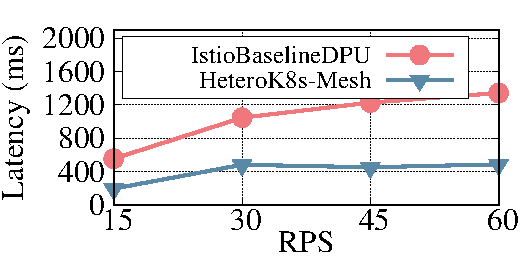
\includegraphics[width=0.98\linewidth]{figs-eval/eval-mesh-scale-p99-eps-converted-to.pdf}\\[-0.4ex]
    \footnotesize\textbf{（e）P99 延迟。}
  \end{minipage}
  \begin{minipage}[t]{0.235\linewidth}
    \centering
    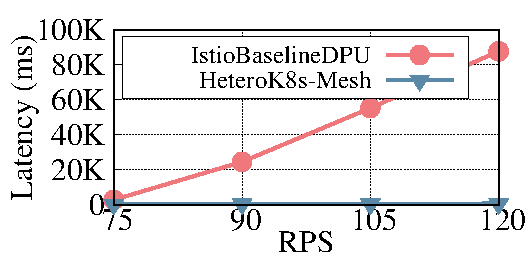
\includegraphics[width=0.98\linewidth]{figs-eval/eval-mesh-scale-p99-large-eps-converted-to.pdf}\\[-0.4ex]
    \footnotesize\textbf{（f）P99 延迟（高 RPS）。}
  \end{minipage}
  \caption{BlueField-2 DPU 上带服务网格的微服务。DeathStar 中 SN 表示 Social Network，HR 表示 Hotel Reservation。图中给出端到端延迟；除非明确说明，单位均为毫秒。}
  \label{fig:eval-mesh-big}
\end{figure*}

\section{\sys：XPU 云原生系统}
\label{s:case}

我们提出 \sys：一个基于 Kubernetes 的云原生系统，它利用 \os 在不同场景下有效且高效地使用 DPU。下面给出三个案例研究：卸载工作节点的基础设施应用（第~\ref{s:case-mesh} 节）、卸载用户应用（第~\ref{s:case-FaaS} 节），以及卸载控制面的基础设施应用（第~\ref{s:case-scheduler} 节）。

\subsection{案例研究：服务网格与微服务}
\label{s:case-mesh}

服务网格是一种代表性模式，它会向每个微服务 Pod 注入一个\emph{边车}容器（代理），从而同时带来资源成本和通信延迟问题。下面说明 \sys 如何利用 \os 优化代理类基础设施容器造成的成本。

\myparagraph{采用 Istio 的基线系统。}
除基本代理设计（图~\ref{fig:intro-wingman}(a)）外，先进服务网格系统 Istio\cite{istio}还支持一种能有效缓解成本的高级体系结构：\emph{waypoint 边车}\cite{istio-ambient}（图~\ref{fig:intro-wingman}(b)）。它把边车解耦成\emph{零信任隧道（ztunnel）}与\emph{waypoint 边车}。ztunnel 可由节点上的全部应用共享，用于执行 L4 策略；waypoint 边车则专用于某个应用、执行 L7 策略，并可被调度到其他节点。解耦能节省应用节点上的资源，但把 waypoint 边车调度到第三台服务器也会增加正常路径的延迟。

\myparagraph{\mesh。}
我们设计 \mesh，使用 \os 把边车高效卸载到 DPU，并在性能和可扩展性之间取得平衡。\mesh 支持两种部署方式：（1）把全部代理相关基础设施容器（ztunnel 和 waypoint）卸载到 DPU，使 CPU 专注运行微服务应用（图~\ref{fig:intro-wingman}(d)）；（2）只把 waypoint 容器卸载到 DPU（图~\ref{fig:intro-wingman}(c)）。当 DPU 设备故障或资源不足时，系统会在 CPU 上启动新的 ztunnel 和 waypoint 容器，以保证微服务可用性和服务质量。如果客户端与服务器微服务位于同一节点，\mesh 会尽可能把 ztunnel 和 waypoint 容器部署在 CPU 上。\mesh 使用 \giptable 支持应用与代理之间的间接通信，并依靠 \gsocket 降低通信延迟。

\myparagraph{方法。}
我们以 DeathStarBench\cite{10.1145/3297858.3304013}和 FunctionBench\cite{kim2019practical}作为微服务部署，并为每个微服务部署一个采用 Envoy 的 Istio waypoint 作为网关，以评估 \mesh 的性能。微服务的全部入站与出站流量都由节点上的 ztunnel 截获和处理。我们将 \mesh 与两个系统比较：IstioCPU 和 IstioBaselineDPU。IstioCPU 只在 CPU 上部署微服务 Pod，在许多情形中代表最佳性能，但不能有效利用 DPU 提高可扩展性。IstioBaselineDPU 基于 Istio 实现，同时在 CPU 和 DPU 上部署微服务 Pod，并优先调度到 DPU；它代表以 Pod 粒度使用 DPU 的既有方法。

\myparagraph{端到端性能。}
我们在 \sys-WP（图~\ref{fig:intro-wingman}(c)）和 \sys-All（图~\ref{fig:intro-wingman}(d)）两种配置下评估微服务的端到端延迟。为单独展示\emph{动态拆分}的收益，此处 \mesh 不使用 \gsocket。

FunctionBench 的评估结果见图~\ref{fig:eval-mesh-big}(a)。与 IstioBaselineDPU 相比，\mesh 可使微服务端到端延迟最多降低 60\%（dd、pyaes、chameleon），并改善全部应用的性能。与仅使用 CPU 相比，只把 waypoint 卸载到 DPU 的 \mesh-WP 带来的端到端延迟开销低于 5\%。把 ztunnel 和 waypoint 都卸载到 DPU 的 \mesh-All 可以节省更多 CPU 资源，其端到端开销在 dd 和 pyaes 上仅为 1\%--2\%，在其余应用上均低于 1\%。\mesh-All 的端到端延迟开销之所以低于 \mesh-WP，是因为服务网格基础设施完全卸载到 DPU 后，CPU 上运行的微服务面临更少的 CPU 和缓存、TLB 等微体系结构资源争用，因而运行时间缩短。

DeathStar 的评估结果见图~\ref{fig:eval-mesh-big}(b)。由于 DeathStar 微服务自身的运行延迟很短，此处不卸载 ztunnel。与 BaselineDPU 相比，\mesh 的延迟改善 29\%--74\%；与 CPU（不卸载时的理想性能）相比，它平均只增加不到 1.2ms 的延迟。

\myparagraph{可扩展性。}
我们比较高密度部署下的可扩展性。具体而言，\mesh 与 IstioBaselineDPU 都使用全部 DPU 资源和大部分 CPU 资源部署 Pod。每个微服务 Pod 都配有一个 waypoint 代理；微服务和 waypoint 实例总数相同，均为 70，分配的资源也相同：每个 waypoint 使用 128MB 内存和 100mCPU，每个应用使用 256MB 内存和 300mCPU。测试用例为 Pyaes，请求通过 Nginx 以随机方式均匀负载均衡到全部微服务。

平均延迟结果见图~\ref{fig:eval-mesh-big}(c)(d)，P99 延迟见图~\ref{fig:eval-mesh-big}(e)(f)。在不同 RPS 下，使用 \mesh 部署的微服务均优于 IstioBaselineDPU，端到端延迟改善 39\%。随着 RPS 上升，基线方案中微服务延迟迅速增长，而 \mesh 方案的延迟保持相对稳定。这说明 \mesh 的可扩展性优于基线。

\begin{figure}[t]
  \centering
  \begin{minipage}[t]{0.48\linewidth}
    \centering
    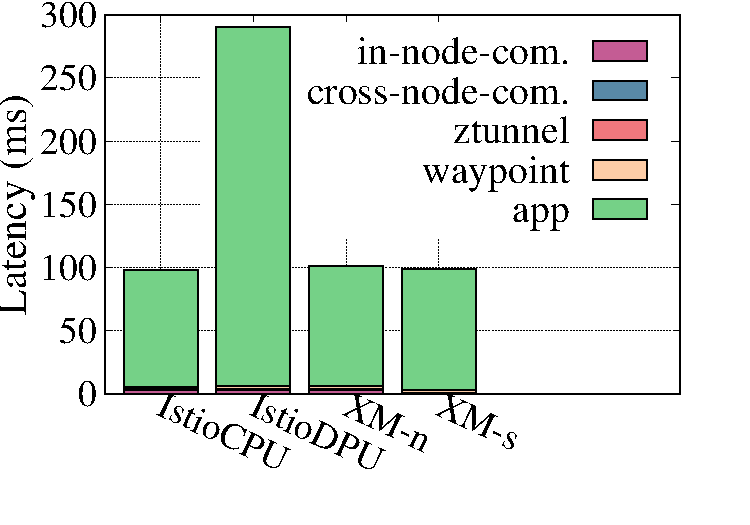
\includegraphics[width=0.98\linewidth]{figs-eval/eval-mesh-breakdown-large-eps-converted-to.pdf}\\[-0.5ex]
    \footnotesize\textbf{（a）大型应用。}
  \end{minipage}
  \begin{minipage}[t]{0.48\linewidth}
    \centering
    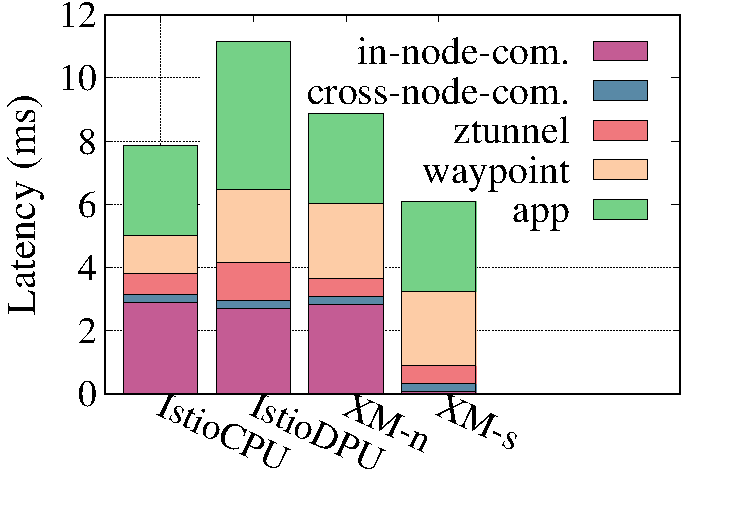
\includegraphics[width=0.98\linewidth]{figs-eval/eval-mesh-breakdown-small-eps-converted-to.pdf}\\[-0.5ex]
    \footnotesize\textbf{（b）小型应用。}
  \end{minipage}
  \caption{BlueField-2 DPU 上的性能分解。XM-n 表示使用 \giptable 的 \mesh，XM-s 表示使用 \gsocket 的 \mesh。}
  \label{fig:eval-mesh-breakdown}
\end{figure}

\myparagraph{性能分解。}
\label{subs:eval-scale}
我们针对大型与小型应用进行性能分解，把端到端延迟拆成五部分：节点内通信（包括 PU 内与跨 PU）延迟、跨节点通信延迟，以及 ztunnel、waypoint 和应用的处理延迟。如图~\ref{fig:eval-mesh-breakdown} 所示，对于大型应用，只采用 \giptable 的 \mesh 已取得良好性能：比 IstioDPU 快 $2\times$，并且几乎与 IstioCPU 相同。此处处理成本占据延迟主导地位，因此 \gsocket 带来的改善很小。对于小型应用，采用 \giptable 的 \mesh 优于 IstioDPU，但 waypoint 延迟上升使其比 IstioCPU 慢 16\%。同时采用 \gsocket 的 \mesh 可通过优化通信进一步降低延迟，性能甚至优于 IstioCPU。

\subsection{案例研究：无服务器计算（FaaS）}
\label{s:case-FaaS}

近期工作\cite{10.1145/3472883.3486972,10.1145/3503222.3507732,copik2022rfaas,wei2022provisioned}已经尝试把 DPU 等异构设备用于无服务器计算，以获得更好的可扩展性和性能，例如 Molecule\cite{10.1145/3503222.3507732}。然而，这些方法通常要求对无服务器运行时和应用都进行不可忽略的修改。

\myparagraph{\faas。}
\sys 在 CPU--DPU 计算机上支持无服务器计算，而且无需修改函数二进制、语言运行时或无服务器运行时（图~\ref{fig:intro-wingman}(e)）。Molecule 使用同一无服务器运行时同时管理 CPU 和 DPU；与之不同，\faas 把不同 PU 视为独立设备，并加入 \os 以透明地实现函数间高效通信。由于 Molecule 的函数采用单容器沙箱，\faas 不使用 \giptable。

我们基于 Molecule 开源的同构实现构建 \faas，并使用其经过修改、支持容器 fork 以降低启动延迟的 runc。\faas 为每个函数实例预加载 \os，但通过\emph{配置文件}只在同一函数链的实例之间启用 \gsocket；单函数应用不会使用 \os。\faas 假设全局网关把一条函数链调度到同一台异构计算机。我们把 \faas 与 Molecule 以及 Molecule-homo（CPU-only 计算机上的同构版本）比较。

\begin{figure}[t]
  \centering
  \begin{minipage}{0.48\linewidth}
    \centering
    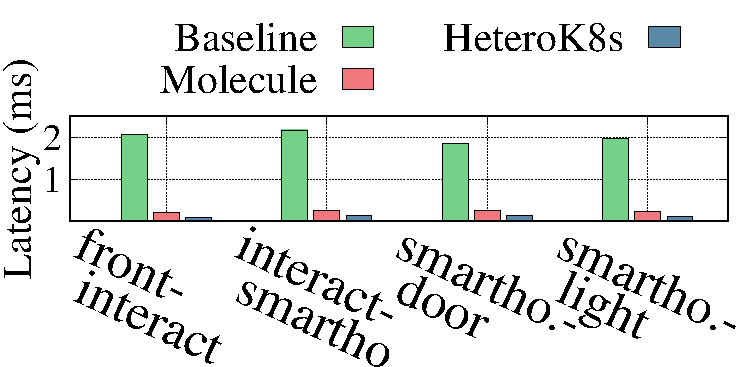
\includegraphics[width=0.98\linewidth]{figs-eval/eval-runtime-micro-dag-host-host-eps-converted-to.pdf}\\[-0.5ex]
    \footnotesize\textbf{（a）CPU 到 CPU}
  \end{minipage}
  \begin{minipage}{0.48\linewidth}
    \centering
    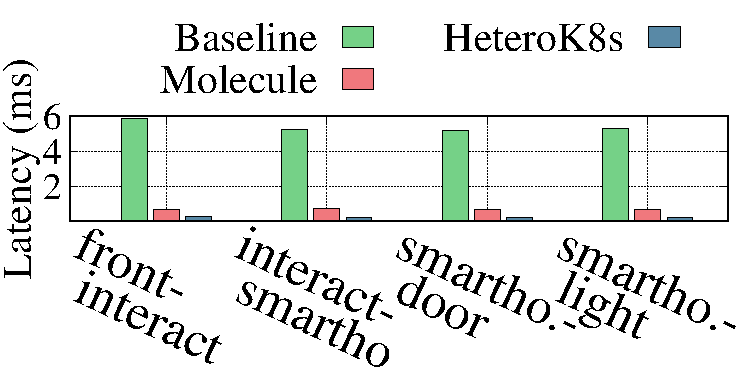
\includegraphics[width=0.98\linewidth]{figs-eval/eval-runtime-micro-dag-NIC-NIC-eps-converted-to.pdf}\\[-0.5ex]
    \footnotesize\textbf{（b）DPU 到 DPU}
  \end{minipage}

  \begin{minipage}{0.48\linewidth}
    \centering
    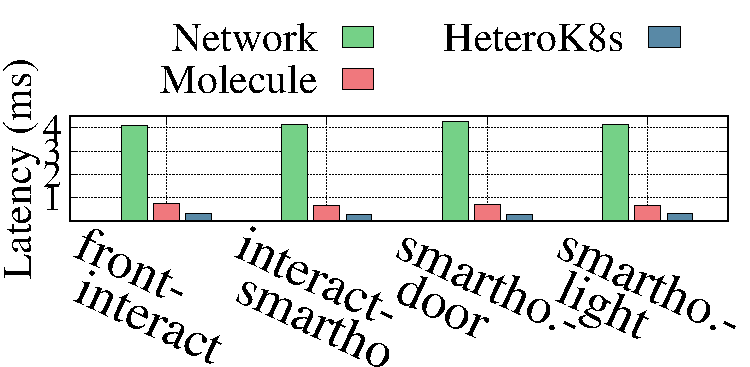
\includegraphics[width=0.98\linewidth]{figs-eval/eval-runtime-micro-dag-host-NIC-eps-converted-to.pdf}\\[-0.5ex]
    \footnotesize\textbf{（c）CPU 到 DPU}
  \end{minipage}
  \begin{minipage}{0.48\linewidth}
    \centering
    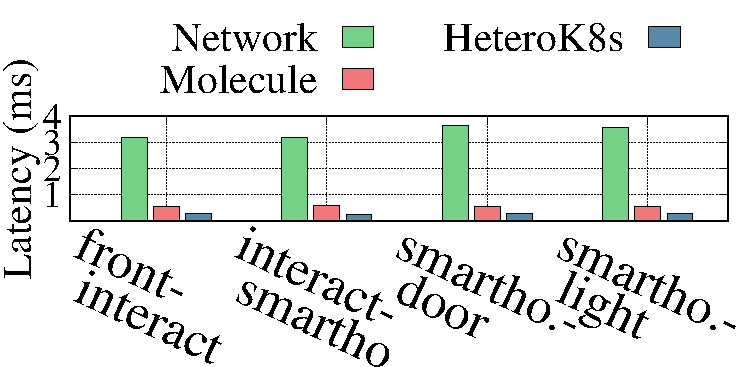
\includegraphics[width=0.98\linewidth]{figs-eval/eval-runtime-micro-dag-NIC-host-eps-converted-to.pdf}\\[-0.5ex]
    \footnotesize\textbf{（d）DPU 到 CPU}
  \end{minipage}
  \caption{无服务器 DAG 通信延迟。相较先进系统 Molecule，\faas 的延迟降低 $2\times$。}
  \label{fig:eval-runtime-micro-dag}
\end{figure}

\myparagraph{微基准。}
我们通过微基准分析一条函数链中两个函数之间的通信延迟。以 Alexa Skills\cite{socc20-serverlessbench}为例，将 \faas 与使用 nIPC 的 Molecule 以及使用 Node.js Express 的基线（Molecule 的同构版本）比较。评估考虑四种情形：仅 CPU、仅 DPU、CPU 到 DPU 和 DPU 到 CPU，结果见图~\ref{fig:eval-runtime-micro-dag}。得益于高效的 nIPC 通信，Molecule 相对基线已经把延迟降低约 $10\times$。\faas 的性能又高约 $2\times$，因为 Molecule 需要额外执行一次 IPC 调用以进入 Hetero-Shim。由于本文实验环境的硬件配置更好，Molecule 的结果优于原论文报告数据\cite{10.1145/3503222.3507732}。

\begin{figure}[t]
  \centering
  \begin{minipage}[t]{0.63\linewidth}
    \centering
    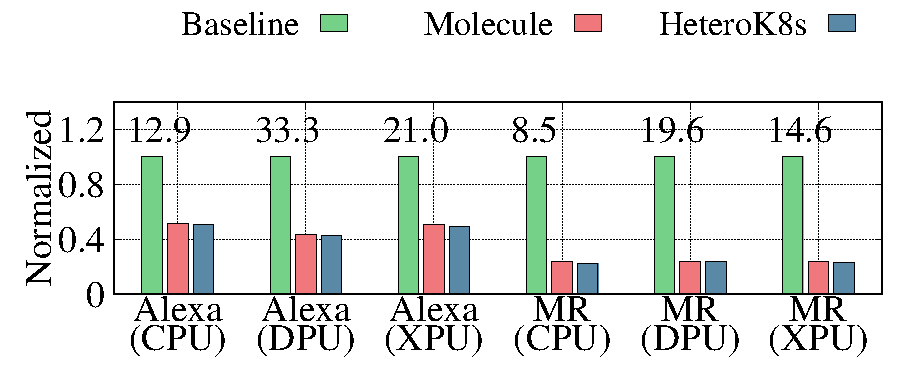
\includegraphics[width=0.98\linewidth]{figs-eval/eval-apps-chain-eps-converted-to.pdf}\\[-0.5ex]
    \footnotesize\textbf{（a）BlueField-2 上的应用}
  \end{minipage}
  \begin{minipage}[t]{0.33\linewidth}
    \centering
    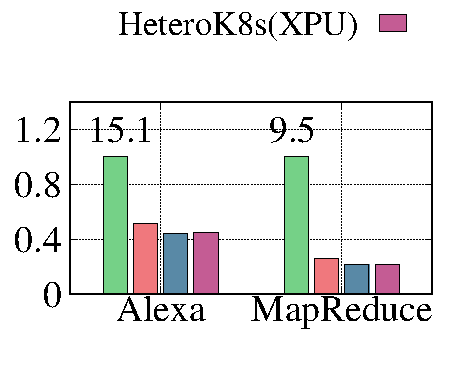
\includegraphics[width=0.98\linewidth]{figs-eval/eval-apps-chain-cxl-eps-converted-to.pdf}\\[-0.5ex]
    \footnotesize\textbf{（b）CXL-DPU 上的应用}
  \end{minipage}
  \caption{链式应用。MR 表示 MapReduce，XPU 表示跨 PU。}
  \label{fig:eval-faas-dag-apps}
\end{figure}

\myparagraph{应用。}
我们分析 ServerlessBench 与 FunctionBench 中两个链式应用 Alexa 和 MapReduce 的端到端延迟。Alexa 包含五个 Node.js 函数，MapReduce 包含三个 Python 函数。我们在 CPU、DPU 和跨 PU 三种情形下比较基线（Molecule-homo）、Molecule 和 \faas。跨 PU 情形保证所有函数间调用都跨越 PU；例如 Alexa 的第 1、3、5 个函数位于主机 CPU，第 2、4 个函数位于 DPU。全部实例均为热启动，不计冷启动成本。结果见图~\ref{fig:eval-faas-dag-apps}。与基线相比，Molecule 在 Alexa 上将端到端延迟降低 $1.94$--$2.32\times$，在 MapReduce 上降低 $4.20$--$4.21\times$；\faas 的延迟进一步改善，在 Alexa 上降低 $1.96$--$2.34\times$，在 MapReduce 上降低 $4.19$--$4.45\times$。

\begin{figure}[t]
  \centering
  \begin{minipage}[t]{0.48\linewidth}
    \centering
    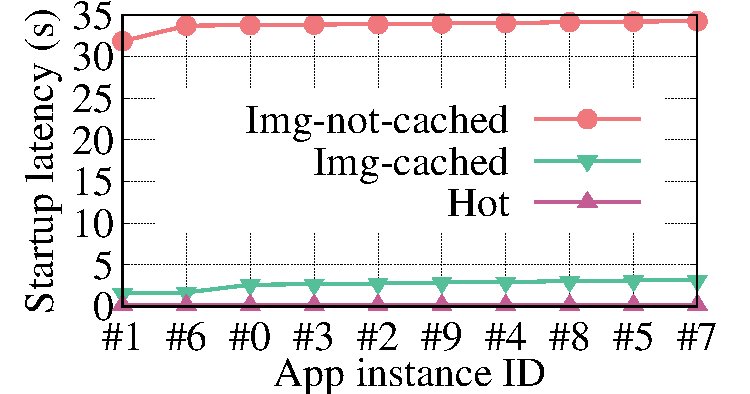
\includegraphics[width=0.98\linewidth]{figs-eval/case-scheduler-motiv-eps-converted-to.pdf}\\[-0.5ex]
    \footnotesize\textbf{（a）动机（Knative）}
  \end{minipage}
  \begin{minipage}[t]{0.48\linewidth}
    \centering
    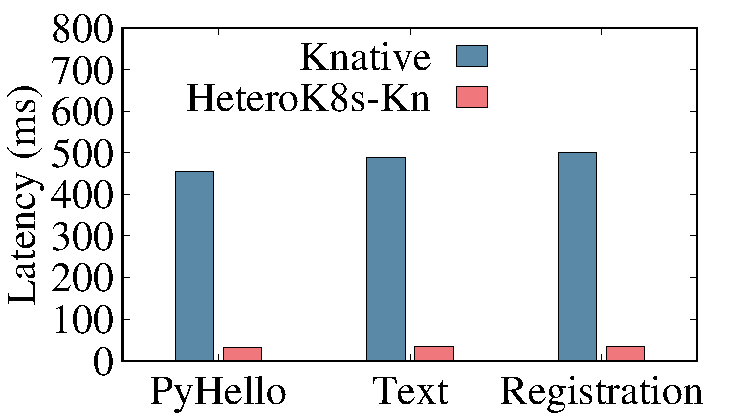
\includegraphics[width=0.98\linewidth]{figs-eval/case-scheduler-opt-eps-converted-to.pdf}\\[-0.5ex]
    \footnotesize\textbf{（b）优化结果}
  \end{minipage}
  \caption{卸载调度器以实现镜像感知调度。}
  \label{fig:eval-scheduler}
\end{figure}

\subsection{案例研究：卸载调度器}
\label{s:case-scheduler}

\myparagraph{动机。}
启动延迟是云原生应用最重要的指标之一\cite{socc20-serverlessbench}。虽然已有许多工作使用检查点/恢复、fork 和缓存来优化容器启动延迟，但我们观察到\emph{镜像拉取}仍带来显著挑战：如果请求被调度到尚未准备相应镜像的节点，平台必须先拉取镜像，再启动实例。为分析这项成本，我们使用 Kperf 在广泛采用的 FaaS 系统 Knative\cite{knative}上评估响应延迟。如图~\ref{fig:eval-scheduler}(a) 所示，镜像未缓存时的延迟约为已缓存时的 $10\times$。

\myparagraph{思路与挑战。}
云原生平台通常依赖全局调度器为请求选择节点，例如 Kubernetes 的 kube-scheduler。一种思路是采用\emph{镜像感知调度器}，优先把请求分配给已经准备好镜像的节点；Kubernetes 就支持镜像局部性策略\cite{image-locality}。然而，这要求调度器维护全部节点的镜像信息。在真实环境中，缓存所有镜像信息需要 1GB--10GB 资源，而且镜像状态更新会通知调度器，使调度器成为控制面瓶颈。

\myparagraph{解决方案。}
\sys 可以把调度器中的镜像缓存卸载到 DPU，利用 DPU 的空余资源维护镜像信息。此外，DPU 更接近网络，由它更新镜像状态也更合理。在此卸载基础上，我们设计了镜像与模板感知策略（容器 fork 的模板见文献\cite{10.1145/3503222.3507732}），并将其实现为 kube-scheduler 插件，优先选择已经具有模板实例和缓存镜像的节点。\sys 通过卸载后的调度器与新策略支持未经修改的 Knative。如图~\ref{fig:eval-scheduler}(b) 所示，我们分析由四台机器组成的完整集群的平均延迟；\sys-Kn 将平均延迟从 481ms 降至 33ms，即降低 $14.4\times$。
